\documentclass{beamer}
\usepackage[utf8]{inputenc}

\usetheme{Madrid}
\usecolortheme{default}
\usepackage{amsmath,amssymb,amsfonts,amsthm}
\usepackage{txfonts}
\usepackage{tkz-euclide}
\usepackage{listings}
\usepackage{adjustbox}
\usepackage{array}
\usepackage{tabularx}
\usepackage{gvv}
\usepackage{lmodern}
\usepackage{circuitikz}
\usepackage{tikz}
\usepackage{graphicx}
\usepackage{multicol}
\setbeamertemplate{page number in head/foot}[totalframenumber]

\usepackage{tcolorbox}
\tcbuselibrary{minted,breakable,xparse,skins}

\definecolor{bg}{gray}{0.95}
\DeclareTCBListing{mintedbox}{O{}m!O{}}{%
	breakable=true,
	listing engine=minted,
	listing only,
	minted language=#2,
	minted style=default,
	minted options={%
		linenos,
		gobble=0,
		breaklines=true,
		breakafter=,,
		fontsize=\small,
		numbersep=8pt,
		#1},
	boxsep=0pt,
	left skip=0pt,
	right skip=0pt,
	left=25pt,
	right=0pt,
	top=3pt,
	bottom=3pt,
	arc=5pt,
	leftrule=0pt,
	rightrule=0pt,
	bottomrule=2pt,
	toprule=2pt,
	colback=bg,
	colframe=orange!70,
	enhanced,
	overlay={%
		\begin{tcbclipinterior}
			\fill[orange!20!white] (frame.south west) rectangle ([xshift=20pt]frame.north west);
	\end{tcbclipinterior}},
}

\lstset{
	language=C,
	basicstyle=\ttfamily\small,
	keywordstyle=\color{blue},
	stringstyle=\color{orange},
	commentstyle=\color{green!60!black},
	numbers=left,
	numberstyle=\tiny\color{gray},
	breaklines=true,
	showstringspaces=false,
}

%------------------------------------------------------------
\title{1.2.72}
\author{RAVULA SHASHANK REDDY - EE25BTECH11047}
\date{}
\begin{document}

\frame{\titlepage}

\begin{frame}{Question}
Evaluate the integral:
\begin{align}
\int_{0}^{3} \int_{0}^{3-x} (6 - x - y)\, dy\, dx
\end{align}

\textbf{Options:}
\begin{itemize}
\item[(a)] 13.5
\item[(b)] 18.0
\item[(c)] 40.5
\item[(d)] 54.0
\end{itemize}
\end{frame}

%-------------------------------------------------

\begin{frame}{Step 1: Inner Integral}
Evaluate the inner integral:
\begin{align}
\int_{0}^{3-x} (6 - x - y)\, dy
\end{align}

Split the integral:
\begin{align}
= \int_{0}^{3-x} (6 - x)\, dy - \int_{0}^{3-x} y\, dy
\end{align}

\begin{align}
= (6 - x)(3 - x) - \frac{(3 - x)^2}{2}
\end{align}
\end{frame}

%-------------------------------------------------

\begin{frame}{Step 2: Simplification}
\begin{align}
(6 - x)(3 - x) &= 18 - 9x + x^2 \\
\frac{(3 - x)^2}{2} &= \frac{9 - 6x + x^2}{2}
\end{align}

\begin{align}
\Rightarrow \int_{0}^{3-x} (6 - x - y)\, dy
&= 18 - 9x + x^2 - \frac{9 - 6x + x^2}{2} \\
&= \frac{27 - 12x + x^2}{2}
\end{align}
\end{frame}

%-------------------------------------------------

\begin{frame}{Step 3: Outer Integral}
\begin{align}
\int_{0}^{3} \frac{27 - 12x + x^2}{2} \, dx
= \frac{1}{2} \int_{0}^{3} (27 - 12x + x^2)\, dx
\end{align}

\begin{align}
= \frac{1}{2} \left[ 27x - 6x^2 + \frac{x^3}{3} \right]_{0}^{3}
\end{align}
\end{frame}

%-------------------------------------------------

\begin{frame}{Step 4: Final Calculation}
Substitute limits:
\begin{align}
= \frac{1}{2} \left( 81 - 54 + 9 \right)
\end{align}

\begin{align}
= \frac{1}{2} \times 36 = 18
\end{align}

\vspace{0.5cm}

\end{frame}

%-------------------------------------------------

\begin{frame}{Region of Integration}

\noindent\textbf{In one line:} Volume under the plane $z = 6 - x - y$ over a triangular region in the $xy$-plane.
\end{frame}

\begin{frame}{ Numerical Grid Squaring Method }

In this method , region is divided into small squares of size:
\begin{align}
h \times h
\end{align}

At each grid point $(x_i, y_j)$, the function value is:
\begin{align}
f(x_i, y_j) = 6 - x_i - y_j
\end{align}

The double integral is approximated as:
\begin{align}
\int_{0}^{3} \int_{0}^{3-x} (6 - x - y)\, dy\, dx
\approx
\sum_{i} \sum_{j} (6 - x_i - y_j)\, h^2
\end{align}

\end{frame}
\begin{frame}{Numerical Grid Squaring Method}

\begin{enumerate}
\item Choose a small step size $h$
\item Loop over $x$ from $0$ to $3$
\item For each $x$, loop over $y$ from $0$ to $3 - x$
\item Accumulate:
\begin{align}
\text{sum} += (6 - x_i - y_j)
\end{align}
\item Multiply final sum by $h^2$
\end{enumerate}
\end{frame}
\begin{frame}[fragile]
\frametitle{Python Code for Grid Squaring Method}

\begin{lstlisting}
import numpy as np

h = 0.001  # step size

x = np.arange(0, 3 + h, h)

total = 0

for xi in x:
    y = np.arange(0, 3 - xi + h, h)
    for yj in y:
        total += (6 - xi - yj)

result = total * h * h

print("Approximate Value =", result)
\end{lstlisting}
\end{frame}
\begin{frame}{Conclusion}

For $h$ = 0.01
\begin{align}
\int_{0}^{3} \int_{0}^{3-x} (6 - x - y)\, dy\, dx
\approx
\sum_{i} \sum_{j} (6 - x_i - y_j)\, h^2 = 18.018831724000133
\end{align}

For a sufficiently small step size $h$, the numerical result is:
\begin{align}
\boxed{18 \text{ (approximately)}}
\end{align}

\section*{Conclusion}

The grid squaring method approximates the double integral by summing contributions over small squares. 
Accuracy improves as the step size $h$ decreases.

\end{frame}
%-------------------------------------------------
\begin{frame}[fragile]
\frametitle{Python Code}
\begin{lstlisting}
    import numpy as np
import matplotlib.pyplot as plt

fig = plt.figure(figsize=(10, 8))
ax = fig.add_subplot(111, projection='3d')

# --- Top surface (plane) ---
x = np.linspace(0, 3, 100)
y = np.linspace(0, 3, 100)
X, Y = np.meshgrid(x, y)

Z = 6 - X - Y
mask = (X + Y <= 3)
Z = np.where(mask, Z, np.nan)

ax.plot_surface(X, Y, Z, alpha=0.7)
\end{lstlisting}
\end{frame}
\begin{frame}[fragile]
\frametitle{Python Code}
\begin{lstlisting}
# --- Bottom (triangle) ---
ax.plot_trisurf(
    [0, 3, 0],
    [0, 0, 3],
    [0, 0, 0],
    alpha=0.4
)

# --- Side 1 (x = 0 plane) ---
y_side = np.linspace(0, 3, 50)
z_side = np.linspace(0, 6, 50)
Y_side, Z_side = np.meshgrid(y_side, z_side)
X_side = np.zeros_like(Y_side)

# Keep only valid region
mask_side = (Z_side <= 6 - Y_side)
Z_side = np.where(mask_side, Z_side, np.nan)

ax.plot_surface(X_side, Y_side, Z_side, alpha=0.4)
\end{lstlisting}
\end{frame}
\begin{frame}[fragile]
\frametitle{Python Code}
\begin{lstlisting}
# --- Side 2 (y = 0 plane) ---
x_side = np.linspace(0, 3, 50)
z_side = np.linspace(0, 6, 50)
X_side, Z_side = np.meshgrid(x_side, z_side)
Y_side = np.zeros_like(X_side)

mask_side = (Z_side <= 6 - X_side)
Z_side = np.where(mask_side, Z_side, np.nan)

ax.plot_surface(X_side, Y_side, Z_side, alpha=0.4)

# Labels
ax.set_xlabel('X')
ax.set_ylabel('Y')
ax.set_zlabel('Z')

ax.set_title('Solid Volume under z = 6 - x - y')

plt.show()
\end{lstlisting}
\end{frame}

\begin{frame}{Plot}
\begin{figure}
    \centering
    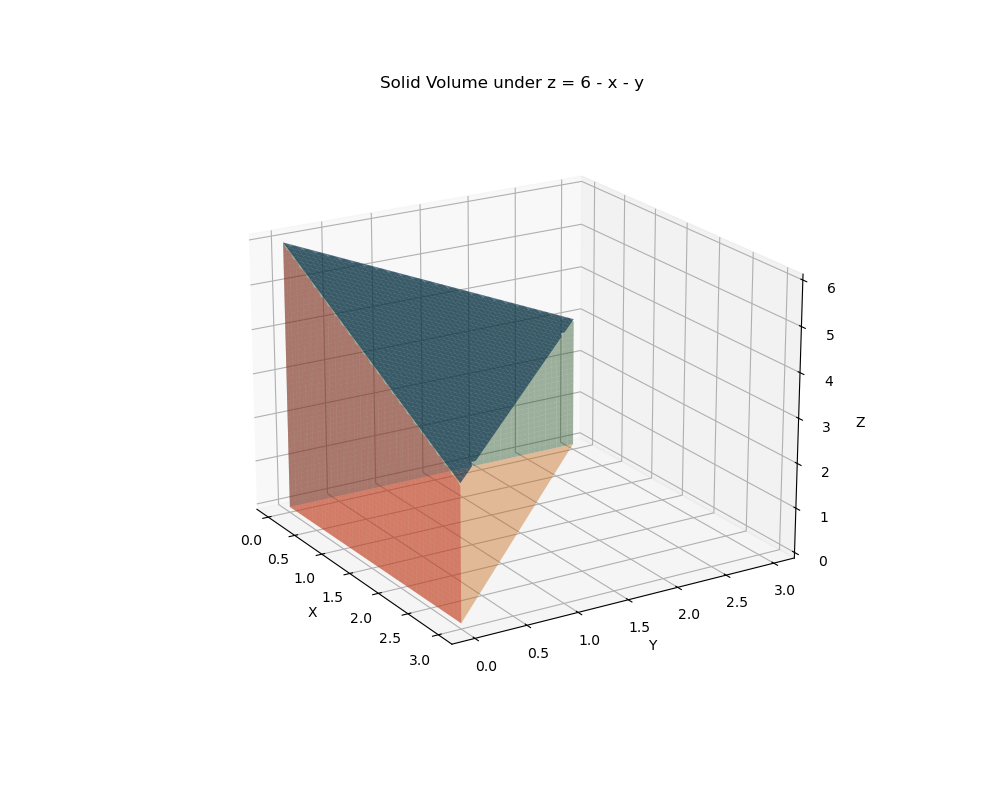
\includegraphics[width=1.0\linewidth]{Figure_1.png}
    \caption{}
    \label{fig:placeholder}
\end{figure}
    
\end{frame}
\end{document}